% Created 2023-04-19 Wed 16:18
% Intended LaTeX compiler: lualatex
\documentclass[11pt]{article}
\usepackage[margin=0.5in]{geometry}
\usepackage{syntax}
\usepackage{pdfpages}
\usepackage[most]{tcolorbox}
\usepackage{etoolbox}
\usepackage{environ}
\AtBeginEnvironment{quote}{\itshape}
\usepackage[ruled]{algorithm2e}
\let\oldtabular\tabular
\let\oldendtabular\endtabular
\NewEnviron{tabular2}[1]{\tcbox[left=0mm, right=0mm, top=0mm, bottom=0mm]{\oldtabular{#1}\BODY\oldendtabular}}
\BeforeBeginEnvironment{minted}{\begin{tcolorbox}[enhanced, breakable, skin first=enhanced, skin middle=enhanced, skin last=enhanced]}%
\AfterEndEnvironment{minted}{\end{tcolorbox}}
\BeforeBeginEnvironment{verbatim}{\begin{tcolorbox}[enhanced, breakable, skin first=enhanced, skin middle=enhanced, skin last=enhanced]}%
\AfterEndEnvironment{verbatim}{\end{tcolorbox}}
\usepackage{graphicx}
\usepackage{longtable}
\usepackage{wrapfig}
\usepackage{rotating}
\usepackage[normalem]{ulem}
\usepackage{amsmath}
\usepackage{amssymb}
\usepackage{capt-of}
\usepackage{hyperref}
\usepackage{minted}
\usepackage{physics}
\author{David Lewis}
\date{\today}
\title{lecture 21}
\hypersetup{
 pdfauthor={David Lewis},
 pdftitle={lecture 21},
 pdfkeywords={},
 pdfsubject={},
 pdfcreator={Emacs 30.0.50 (Org mode 9.6.1)}, 
 pdflang={English}}
\begin{document}

\maketitle

\section*{1.}
\label{sec:org3b51ef3}
\subsection*{a.}
\label{sec:orgc5f8614}
\begin{minted}[fontsize=\scriptsize,breaklines=true,breakanywhere=true]{python}
D = [1, 2, 3, 3, 3, 4, 6, 7, 8, 8, 8, 9]
unique = set(D)
counts = {}
for i in unique:
    count = 0
    for k in D:
        if i == k:
            count+=1
    counts[i] = count

rel_freq = []
for key, value in counts.items():
    rel_freq.append(value/len(D))
total = 0
CDF = []
for i in rel_freq:
    CDF.append(i+total)
    total+=i
CDF
\end{minted}
\subsection*{b.}
\label{sec:org84179a1}
\begin{minted}[fontsize=\scriptsize,breaklines=true,breakanywhere=true]{python}
import matplotlib.pyplot as plt
fig, ax = plt.subplots()
ax.step(list(unique), CDF)
plt.show()
\end{minted}

\begin{center}
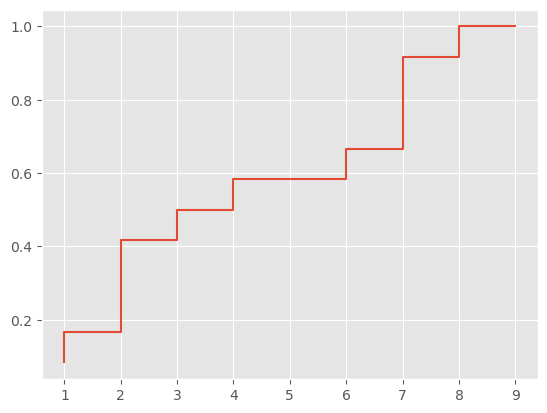
\includegraphics[width=0.7\textwidth]{test.png}
\end{center}
\subsection*{c.}
\label{sec:org11f7b70}
\(f(x,h) = \frac{F(x+h/2)- F(x-h/2)}{h}\)

\begin{minted}[fontsize=\scriptsize,breaklines=true,breakanywhere=true]{python}
F = dict(zip(list(unique), CDF))
# add missing values to step function (quick hack)
F[0] = 0
F[5] = F[4]
F[10] = F[9]
F[11] = F[9]
F[12] = F[9]
F[-1] = F[0]
F[-2] = F[0]
F[-3] = F[0]

from math import floor
def f(x, h):
    #print(F[floor(x+h/2)], F[floor(x-h/2)])
    return (F[floor(x+h/2)] - F[floor(x-h/2)])/h

h_1 = [f(x, 1) for x in range(0,11)]
h_1
\end{minted}
\subsection*{d.}
\label{sec:orge5d883c}
\begin{minted}[fontsize=\scriptsize,breaklines=true,breakanywhere=true]{python}
h_5 = [f(x, 5) for x in range(0,11)]
h_5
\end{minted}
\subsection*{e.}
\label{sec:orga7503f3}
\begin{minted}[fontsize=\scriptsize,breaklines=true,breakanywhere=true]{python}
import matplotlib.pyplot as plt
fig, (ax1, ax2) = plt.subplots(2)
ax1.step(range(0,11), h_1)
ax2.step(range(0,11), h_5)
plt.show()
\end{minted}
\subsection*{f.}
\label{sec:orgd8a7293}
I would expect that the above plot would dip into the negative, as it appears to
be a visualization of the changes in the step (empirical cumulative
distribution) kernel.
\section*{2.}
\label{sec:org238ac5f}
\begin{itemize}
\item CBAD
\item the higher the h, the smoother the distribution
\end{itemize}
\section*{3.}
\label{sec:orga576ef4}
\subsection*{a.}
\label{sec:orgf44e737}
\begin{equation*}
\nabla f(x) = \frac{1}{nh^{d+2}}\sum \limits^n_{i=1}K\left(\frac{x-x_i}{h}\right)(x_i-x)
\end{equation*}

\begin{itemize}
\item \(K(\frac{x-x_i}{h})\) is the kernel term (a scalar value). Inversely
proportional to distance in the gaussian case.
\item \((x_i-x)\) is a vector that makes up a portion of the gradient. All of these
vectors summed together is the gradient.
\end{itemize}
\subsection*{b.}
\label{sec:org101d391}
Because A is closer to the marked location, it will have a greater affect on the
direction of the gradient. This is because the Kernel term is inversely
proportional to the distance.

\subsection*{c.}
\label{sec:orgd53055f}
\begin{equation}
x^{t+1} = x^t + \delta \frac{\nabla f(x)}{\|\nabla f(x) \|}
\end{equation}

\begin{itemize}
\item Since A has a greater effect, the gradient vector will be to the peak by A
rather than the peak by B. Since \(x^t\) moves in the direction of the
gradient vector (by step \(\delta\)) to get to \(x^{t+1}\).
\end{itemize}
\end{document}